%  LaTeX support: latex@mdpi.com 
%  In case you need support, please attach all files that are necessary for compiling as well as the log file, and specify the details of your LaTeX setup (which operating system and LaTeX version / tools you are using).

% You need to save the "mdpi.cls" and "mdpi.bst" files into the same folder as this template file.

%=================================================================
\documentclass[sensors,article,submit,moreauthors,pdftex,10pt,a4paper]{mdpi} 
%
%--------------------
% Class Options:
%--------------------
% journal
%----------
% Choose between the following MDPI journals:
% actuators, admsci, aerospace, agriculture, agronomy, algorithms, animals, antibiotics, antibodies, antioxidants, applsci, arts, atmosphere, atoms, axioms, batteries, behavsci, beverages, bioengineering, biology, biomedicines, biomimetics, biomolecules, biosensors, brainsci, buildings, carbon, cancers, catalysts, cells, challenges, chemosensors, children, chromatography, climate, coatings, computation, computers, condensedmatter, cosmetics, cryptography, crystals, data, dentistry, designs, diagnostics, diseases, diversity, econometrics, economies, education, electronics, energies, entropy, environments, epigenomes, fermentation, fibers, fishes, fluids, foods, forests, futureinternet, galaxies, games, gels, genealogy, genes, geosciences, geriatrics, healthcare, horticulturae, humanities, hydrology, informatics, information, infrastructures, inorganics, insects, instruments, ijerph, ijfs, ijms, ijgi, ijtpp, inventions, jcdd, jcm, jdb, jfb, jfmk, jimaging, jof, jintelligence, jlpea, jmse, jpm, jrfm, jsan, land, languages, laws, life, literature, lubricants, machines, magnetochemistry, marinedrugs, materials, mathematics, mca, mti, medsci, medicines, membranes, metabolites, metals, microarrays, micromachines, microorganisms, minerals, molbank, molecules, mps, nanomaterials, ncrna, neonatalscreening, nutrients, particles, pathogens, pharmaceuticals, pharmaceutics, pharmacy, philosophies, photonics, plants, polymers, processes, proteomes, publications, recycling, religions, remotesensing, resources, risks, robotics, safety, scipharm, sensors, separations, sexes, sinusitis, socsci, societies, soils, sports, standards, sustainability, symmetry, systems, technologies, toxics, toxins, tropicalmed, universe, urbansci, vaccines, vetsci, viruses, water
%---------
% article
%---------
% The default type of manuscript is article, but can be replaced by: 
% addendum, article, book, bookreview, briefreport, casereport, changes, comment, commentary, communication, conceptpaper, correction, conferenceproceedings, conferencereport, expressionofconcern, meetingreport, creative, datadescriptor, discussion, editorial, essay, erratum, hypothesis, interestingimage, letter, newbookreceived, opinion, obituary, projectreport, reply, retraction, review, preprints, shortnote, supfile, technicalnote
% supfile = supplementary materials
%----------
% submit
%----------
% The class option "submit" will be changed to "accept" by the Editorial Office when the paper is accepted. This will only make changes to the frontpage (e.g. the logo of the journal will get visible), the headings, and the copyright information. Also, line numbering will be removed. Journal info and pagination for accepted papers will also be assigned by the Editorial Office.
%------------------
% moreauthors
%------------------
% If there is only one author the class option oneauthor should be used. Otherwise use the class option moreauthors.
%---------
% pdftex
%---------
% The option pdftex is for use with pdfLaTeX. If eps figure are used, remove the option pdftex and use LaTeX and dvi2pdf.

%=================================================================
\firstpage{1} 
\makeatletter 
\setcounter{page}{\@firstpage} 
\makeatother 
\articlenumber{x}
\doinum{10.3390/------}
\pubvolume{xx}
\pubyear{2016}
\copyrightyear{2016}
\externaleditor{Academic Editor: name}
\history{Received: date; Accepted: date; Published: date}

%------------------------------------------------------------------
% The following line should be uncommented if the LaTeX file is uploaded to arXiv.org
%\pdfoutput=1

%=================================================================
% Add packages and commands here. The following packages are loaded in our class file: fontenc, calc, indentfirst, fancyhdr, graphicx, lastpage, ifthen, lineno, float, amsmath, setspace, enumitem, mathpazo, booktabs, titlesec, etoolbox, amsthm, hyphenat, natbib, hyperref, footmisc, geometry, caption, url, mdframed

\usepackage{amsfonts}
\usepackage{stmaryrd}
\usepackage{xspace}
\usepackage{tikz}
\usepackage{pgfplots}
\usepackage{subcaption}

\usetikzlibrary{patterns}
\pgfplotsset{width=12cm,compat=1.14}
\usetikzlibrary{arrows,shapes,positioning,shadows,trees,shapes.geometric}
\newcommand{\degree}{\ensuremath{{}^{\circ}}\xspace}
%=================================================================
%% Please use the following mathematics environments: Theorem, Lemma, Corollary, Proposition, Characterization, Property, Problem, Example, ExamplesandDefinitions, Remark, Definition
%% For proofs, please use the proof environment (the amsthm package is loaded by the MDPI class).

%=================================================================
% Full title of the paper (Capitalized)
\Title{Hybrid Orientation Based Human Limbs Motion Tracking Method}

% If this is an expanded version of a conference paper, please cite it here: enter the full citation of your conference paper, and add $\dagger$ in the end of the title of this article.
%\conference{}

% Authors, for the paper (add full first names)
\Author{Grzegorz Glonek $^{1,\dagger,*}$ and Adam Wojciechowski $^{1,\dagger}$}
% Authors, for metadata in PDF
\AuthorNames{Grzegorz Glonek and Adam Wojciechowski}

% Affiliations / Addresses (Add [1] after \address if there is only one affiliation.)
\address{%
$^{1}$ \quad Institute of Information Technology, Faculty of Technical Physics, Information Technology and Applied Mathematics, Lodz University of Technology, Wolczańska 215, 90-924 Lodz, Poland}

% Contact information of the corresponding author
\corres{Correspondence: grzegorz@glonek.net.pl; Tel.: +48-660-758-666}

% Current address and/or shared authorship
\firstnote{These authors contributed equally to this work.} 

% Simple summary
%\simplesumm{}

% Abstract (Do not use inserted blank lines, i.e. \\) 
\abstract{One of the key technologies that lays behind human-machine interaction is limbs motion tracking. To make the interaction effective, the motion tracking must be able to estimate precise and unambiguous position of each tracked human joint and body part. In recent years, motion tracking became very popular and broadly available for home users because of an easy access to cheap and robust tracking devices. The paper defines the novel approach to data fusion for two of such cheap tracking devices: Microsoft Kinect v.1 and inertial measurement units (IMU). The detailed review of their working characteristics leads to the description of the method that fuses data from both devices and, at the same time, compensates their imprecisions. The paper also presents the series of performed experiments that verified the method's' accuracy. This novel approach allowed improving the precision of joints positioning up to 18\%, in terms of the most relevant methods described in the literature.}

% Keywords
\keyword{data fusion;Microsoft Kinect;IMU;motion tracking}

% The fields PACS, MSC, and JEL may be left empty or commented out if not applicable
%\PACS{J0101}
%\MSC{}
%\JEL{}
%\AMS{}

%%%%%%%%%%%%%%%%%%%%%%%%%%%%%%%%%%%%%%%%%%
% Only for the journal Data:

%\dataset{DOI number or link to the deposited data set in cases where the data set is published or set to be published separately. If the data set is submitted and will be published as a supplement to this paper in the journal Data, this field will be filled by the editors of the journal. In this case, please make sure to submit the data set as a supplement when entering your manuscript into our manuscript editorial system.}

%\datasetlicense{license under which the data set is made available (CC0, CC-BY, CC-BY-SA, CC-BY-NC, etc.)}

%%%%%%%%%%%%%%%%%%%%%%%%%%%%%%%%%%%%%%%%%%
% For Conference Proceedings Papers: add the conference title here
%\conferencetitle{}

%\setcounter{secnumdepth}{4}
%%%%%%%%%%%%%%%%%%%%%%%%%%%%%%%%%%%%%%%%%%
\begin{document}

%%%%%%%%%%%%%%%%%%%%%%%%%%%%%%%%%%%%%%%%%%
%% Only for the journal Gels: Please place the Experimental Section after the Conclusions

%%%%%%%%%%%%%%%%%%%%%%%%%%%%%%%%%%%%%%%%%%
%\setcounter{section}{-1} %% Remove this when starting to work on the template.
%\section{How to Use this Template}
%The template details the sections that can be used in a manuscript. Note that the order of article sections may differ from the requirements of the journal (e.g. for the positioning of the Materials and Methods section). Please check the instructions for authors page of the journal to verify the correct order. For any questions, please contact the editorial office of the journal or support@mdpi.com. For LaTeX related questions please contact Janine Daum at latex-support@mdpi.com.

\section{Introduction}

%The introduction should briefly place the study in a broad context and highlight why it is important. It should define the purpose of the work and its significance. The current state of the research field should be reviewed carefully and key publications cited. Please highlight controversial and diverging hypotheses when necessary. Finally, briefly mention the main aim of the work and highlight the principal conclusions. As far as possible, please keep the introduction comprehensible to scientists outside your particular field of research. Citing a journal paper \cite{ref-journal}. And now citing a book reference \cite{ref-book}.
Human limbs motion tracking can be defined as a process of unambiguous limbs joints spatial positioning, devoid of significant delays. Nowadays, it might be exploited within several areas, such as entertainment issues, virtual environments interaction or medical rehabilitation treatment. However, it is the system precision that determines its possible application. \\
Since 1973, when Gunnar Johanson invented his motion capture system \cite{Johansson1973}, such techniques were available mainly for professionals. However, since 2010, when Microsoft Company released Kinect v.1 controller, motion capture became available to almost everyone. Microsoft Kinect controller is an exemplary implementation of the optical, markerless motion capture system. Though it was designed for and mainly used in the field of home physical activity games, Kinect became a popular subject for many researchers, whose goal was to find other, more advanced scenarios, where this controller might be applied \cite{Lange2012, Chang2011}.

An easy access to the motion capture has been additionally supplemented and magnified by the fact that inertial devices such as gyroscopes and accelerometers (IMU – inertial measurement units) have become an integral and mandatory part of current electronic devices. These units are built in every smartphone device and they are used in various applications like pedometers \cite{Huang2012, Jayalath2013}, screen rotators \cite{Pedley2013} or digital camera orientation detectors.

Inertial measurement units (IMU) are also used as measuring devices in non-optical inertial human limbs motion tracking systems i.e. XSense\footnote{Xsens Motion Technologies, \textit{Products - Xsens 3D motion tracking},\url{https://www.xsens.com/products/}}. Despite IMU, used in products available for home users, being improved continuously, their measurements precision and work limitations can be recognized as blockers for motion capture scenarios that require high accuracy of joints positioning.\\%
The broad and easy access to mentioned devices became a trigger for many researchers around the world to work on these controllers' data fusion methods that would increase the accuracy of joints positioning. Bo et al. \cite{Bo2011a} focused on the knee joint angle estimation. They proposed accelerometer and gyroscope data fusion, with linear Kalman filter, to calculate the angle, and then aligned it to the Kinect’s estimation. In this approach, Kinect's measurements are treated as reference data. Destelle et al. \cite{Destelle2014} have proposed the method based mainly on IMU devices. In this method, the bones orientations and overall pose of the skeleton model has been estimated basing on inertial data only, and sizes of each skeleton bone were set basing on Kinect estimation. Also the skeleton placement was defined by the selected joint position of the Kinect's originated skeleton model. The data from the accelerometer, gyroscope and magnetometer were fused with Madgwick’s filter \cite{Madgwick2011}. In Destelle's method, the role of the Kinect was reduced to only two functions: measuring the initial length of bones and tracking the location of the user on the scene. The pose of the user is estimated only by IMU. Kalkbrenner et al. \cite{Kalkbrenner2014} proposed to combine together the Madgwick’s filter with the linear Kalman filter. In their approach they fused accelerometer and gyroscope data with Madgwick’s filter to estimate the selected bones orientation. Basing on this information and on the bone length, estimated by Kinect, joints positions were calculated. In Kalkbrenner's approach, bone lenghts are taken from Kinect's data in every measurement frame. That means this value is dynamic and may differ few centimeters between two consequitive frames. In the last step joints positions, estimated by Kinect simultaneously, were fused by means of linear Kalman filter with joints positions, estimated with IMU orientations. The Kalkbrenner's method is the method with the highest declared precision of the joints position estimation. Published results show the postiion estimation error about $2.2cm$. In the method proposed by Feng and Murray-Smith \cite{Murray-Smith2014} the accelerometer data has been fused with Kinect measurements with the linear Kalman filter, modified by authors to work with frequency unaligned signals. Publicly available and described results of the Murray-Smith method show that the proposed approach allows to stabilize joints position estimation, at the beginning or at the end of the movement, much faster than the classical Kalman filter implementation. On the othe hand, published diagrams show results in a short time period (no longer than 5s), so it is difficult to define the possitioning accuracy of this method. Tannous et al. \cite{Tannous2016} proposed the extended Kalman filter to fuse bones orientations estimated both by Kinect and IMU devices. 

The analyzis of the available literature show that the majority of known data fusion methods, is based on different variants of Kalman filter (linear, extended or unscented variant), to fuse accelerometer with gyroscope data as well as IMU data with these provided by the Kinect device. Only Kalkbrenner et al. decided to fuse accelerometer and gyroscope data with the Madgwick's filter, which is designed especially for this kind of data and, regarding to the Madgwick's report \cite{Madgwick2011}, it has better accuracy and performance than the linear Kalman filter. It is also noticeable that authors of these methods are selectively taking into consideration characteristics and limitations of measurement devices. As an example, Bo et al. \cite{Bo2011a} and Destelle et al. \cite{Destelle2014} focused mainly on IMU devices and their fusion, treating Kinect device data as a reliable reference for their methods, despite the known inaccuracy of this device. Other mentioned authors compensated some Kinect's measurement problems using proper parameters in the Kalman filter. However, they focused only on joints position estimation fluctuations, ie. Kalkbrenner recalculated fusion parameters only when the difference in the selected joint position estimation value between two consequtive measurement frames was greater than $15cm$. None of the authors included in their methods any compensation of IMU and Kinect's measurement inacuracy due to the environment conditions (the device operational temperature) or the context of the performed motion (the body rotation angle to the camera, the distance from the measurement device). The fact that this kind of factors influence noticably the quality and accuracy of data measured by both devices, may have impact on the further data processing and on the final joint's position estimation.

This paper presents the novel approach to Microsoft Kinect and IMU data fusion that systemically makes up for limitations of both measurement devices and compensates their imperfections also identified and described in this article. The novel orientation based, human limbs’ joints positions tracking method outperforms state-of-art hybrid systems accuracy by 18\%.

%%%%%%%%%%%%%%%%%%%%%%%%%%%%%%%%%%%%%%%%%%
\section{Materials and Methods}

%Materials and Methods should be described with sufficient details to allow others to replicate and build on published results. Please note that publication of your manuscript implicates that you must make all materials, data, computer code, and protocols associated with the publication available to readers. Please disclose at the submission stage any restrictions on the availability of materials or information. New methods and protocols should be described in detail while well-established methods can be briefly described and appropriately cited.

%Research manuscripts reporting large datasets that are deposited in a publicly available database should specify where the data have been deposited and provide the relevant accession numbers. If the accession numbers have not yet been obtained at the time of submission, please state that they will be provided during review. They must be provided prior to publication.

%Interventionary studies involving animals or humans, and other studies require ethical approval must list the authority that provided approval and the corresponding ethical approval code. 
\subsection{Microsoft Kinect controller characteristics}
Microsoft Kinect controller might be described as a RGB-D camera. The first version of this device, originally designed for Xbox 360 video game console, was built from two CMOS cameras and an integrated infrared (IR) projector. One of these CMOS cameras was responsible for an RGB signal and the second one was calibrated to record IR beam’s view. Considering limbs motion tracking and body gesture recognition, the most crucial part of Microsoft Kinect controller is the chip made by the PrimeSense company. All recognition algorithms that stand behind Kinect’s motion tracking, were implemented as a firmware of this processing unit. 
The Microsoft Company has not revealed any detailed description of tracking algorithms and key characteristics, so their retrieval became a subject for scientists and hobbyist \cite{Skalski2015,Gonzalez-Jorge2013,Khoshelham2012}. The good understanding of the Kinect controller constraints seems to be indispensable to create an accurate method that would fuse its data with data collected from any other source. 

In the official device specification it is claimed that the operating range of Kinect varies between $0.8m$ and $4m$ with the field of view $57\degree$ horizontally (fig. \ref{fig:kinect:range:a}) and $43\degree$ vertically (fig. \ref{fig:kinect:range:b}). At the same time, the specification does not reveal the possible heterogeneity of the measurement's accuracy. However, the experiments conducted by the authors showed that there are distance measurement nonlinearities within the Kinect’s working area. Moreover, researchers \cite{DiFilippo2015} and hobbyists\footnote{Stackoverflow Community, \textit{Precision of the kinect depth camera}, \url{https://goo.gl/x4jWoX}} reported that the operating range is different among device series.  

A comparison of fluently changing distances between Kinect and limbs' joints, collected simultaneously from Microsoft Kinect controller and Vicon\footnote{Vicon -- high accuracy, optical marker-based motion capture system.} motion capture system, showed that Kinect has tendencies to underestimate the distance in the close range and to overestimate it in the far range. Collected values (squares on fig. \ref{fig:kinect:distanceAccuracy}) allowed to elaborate distance estimation error function in a form of 3rd order polynomial, as it is presented in eq. \ref{eq:kinect:distanceErrorModel}, calculated basing on eq. \ref{eq:characteristics:kinect:distanceAccuracyPoly}, where $X$ is the matrix of sample points, $Y$ is the matrix of values in these sample points and $A$ is the coefficients matrix used in eq. \ref{eq:kinect:distanceErrorModel}. 

\begin{equation}
	f(z)=0.02z^3-0.11z^2+0.27z-0.25 
	\label{eq:kinect:distanceErrorModel}
\end{equation}

\begin{equation}
\begin{split}
		X^TXA &= X^TY => \begin{bmatrix}
		x_1^0&x_1^1&x_1^2&x_1^3\\
		x_2^0&x_2^1&x_2^2&x_2^3\\
		x_3^0&x_3^1&x_3^2&x_3^3\\
		\dots\\
		x_n^0&x_n^1&x_n^2&x_n^3
		\end{bmatrix}^T
		\begin{bmatrix}
			x_1^0 & x_1^1 & x_1^2 & x_1^3 \\
			x_2^0 & x_2^1 & x_2^2 & x_2^3 \\
			x_3^0 & x_3^1 & x_3^2 & x_3^3 \\
			\dots\\
			x_n^0 & x_n^1 & x_n^2 & x_n^3 
		\end{bmatrix}
		\begin{bmatrix}
			a_0 \\a_1\\a_2\\a_3
		\end{bmatrix}
		=
		\begin{bmatrix}
			x_1^0 & x_1^1 & x_1^2 & x_1^3 \\
			x_2^0 & x_2^1 & x_2^2 & x_2^3 \\
			x_3^0 & x_3^1 & x_3^2 & x_3^3 \\
			\dots\\
			x_n^0 & x_n^1 & x_n^2 & x_n^3 
		\end{bmatrix}^T
		\begin{bmatrix}
			y_0 \\y_1\\y_2\\\dots\\y_n
		\end{bmatrix} 
	\end{split}
\label{eq:characteristics:kinect:distanceAccuracyPoly}
\end{equation}

\begin{figure}[H]
	\centering
	\begin{subfigure}[b]{0.4\textwidth}
		\centering
		\input{Figure1a.tex}
		\caption{Horizontal}
		\label{fig:kinect:range:a}
	\end{subfigure} \hfill
	\begin{subfigure}[b]{0.4\textwidth}
		\centering
		\input{Figure1b.tex}
		\caption{Vertical}
		\label{fig:kinect:range:b}
	\end{subfigure} \hfill
	\begin{subfigure}[p]{0.18\textwidth}
		\hfill
		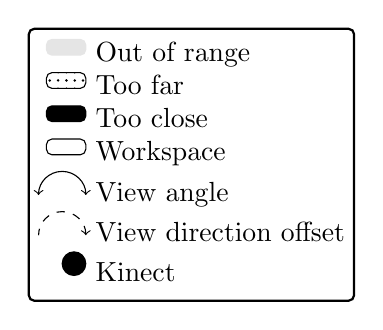
\begin{tikzpicture}[scale=0.2]	
	\node[draw=black,thick,rounded corners=2pt,below left=2mm] {%
		\begin{tabular}{@{}r@{ }l@{}}
			\raisebox{2pt}{\tikz{\draw[black!10, fill=black!10] (0,0) rectangle (5mm,2mm);}}                   & Out of range          \\
			\raisebox{2pt}{\tikz{\draw[black,pattern=dots, pattern color = black] (0,0) rectangle (5mm,2mm);}} & Too far               \\
			\raisebox{2pt}{\tikz{\draw[black, fill=black] (0,0) rectangle (5mm,2mm);}}                         & Too close             \\
			\raisebox{2pt}{\tikz{\draw[black,fill=white] (0,0) rectangle (5mm,2mm);}}             			   & Workspace             \\
			\raisebox{2pt}{\tikz{\draw[<->, thin] (0:0) arc (0:180:0.3);}}                                     & View angle            \\
			\raisebox{2pt}{\tikz{\draw[<-, thin, dashed] (0:0) arc (0:180:0.3);}}                              & View direction offset \\
			\raisebox{2pt}{\tikz{\draw[fill=black] (0, 0) circle (0.15);}}                                     & Kinect                
		\end{tabular}};	
\end{tikzpicture}		
               
	\end{subfigure}
	\caption{Microsoft Kinect v.1 operating range diagram in horizontal (a) and vertical (b) directions}
	\label{fig:kinect:range}
\end{figure}   

Figure \ref{fig:kinect:distanceAccuracy} presents the plot of function defined with eq. \ref{eq:kinect:distanceErrorModel}. The analysis of this chart shows that Kinect’s distance estimation is optimal when the user stands about $2m$ from the device ($2m$ – $2.3m$). Outside this distance range, when Kinect works with a noticeable error, the systematic sensor depth correction should be taken into consideration.

\begin{figure}[H]
	\centering	
	\input{Figure2.tex}										
	\caption{Microsoft Kinect depth measurement accuracy as a function of Kinect-joints distance.}
	\label{fig:kinect:distanceAccuracy}
\end{figure}

Such inaccuracy and its tendencies are probably caused by the algorithm implemented in the Kinect controller. Though Microsoft did not reveal any precise technical description of their method for measuring distance between the camera and objects at the scene, original patent forms \cite{patent:20100118123,patent:20100020078,patent:20080106746} owned by PrimeSense, combined with independent research results\footnote{Andreas Reichinger, \textit{Kinect pattern uncovered}, \url{https://goo.gl/DOqRxZ}}, provide some general overview of how this recognition algorithm works. It is known that the analyzed scene, in front of the Kinect controller, is enlighten with IR light dots structured pattern, which is skew symmetric, so the Kinect can work upright or upside down. Then Kinect analysis the IR pattern’s dots distortion, and basing on that it estimates the subject distance. For the depth map reconstruction, Kinect uses two techniques in parallel: dots blurriness analysis \cite{Fofi2004} and stereo-vision based on a single IR camera and a projector \cite{Rzeszotarski2006}. The achieved depth map is a foundation of a human skeleton estimation algorithm. Depth-retrieved human body parts estimations are subsequently classified into body poses by means of the machine learning approach: random decision forest algorithms as well as on object detection algorithms, such as the one proposed by Viola-Jones \cite{Shotton2008, Shotton2011a}. 

As the only source of data for that estimation process is an IR camera (RGB camera is not used at all), the observed scene must be free of any external source of the IR light. This requirement restricts the usage of Kinect in outdoor scenarios. A need for the scene isolation from any IR sources other than the Kinect itself, is the main reason why Microsoft does not recommend using two or more controllers simultaneously. Nevertheless, scientists invented and published methods on combining signals from several Kinect devices \cite{Asteriadis2013,Kitsikidis2011,Schroder2011}. It is noticeable that information gathered from the Kinect is uncomplete, due to the lack of information about joints rotation along the bone. This is the result of the skeleton model design, where each of 20 tracked joints is described as a single point.

The last major flaw of Microsoft Kinect controller is occlusion, which occurs when a part of user’s body is covered by another object or is hidden behind any other body part (self-occlusion). The occlusion by an external object seems obvious and does not require any additional explanation, however self-occlusions are less intuitive. They are connected with Kinect’s sensitivity to user’s rotation to the camera ($\alpha$ angle in fig. \ref{fig:kinect:rotationAngle}), as Microsoft recommends working with Kinect in the face off pose, which is not precisely defined. Self-performed experiments allowed observing $\alpha$ angle changes while user rotated in front of the camera. Assuming that $P_{Sh_L} = [p^K_{{Sh}_L,X} , p^K_{{Sh}_L,Z}]$ is the position of the left shoulder and $P_{Sh_R} = [p^K_{{Sh}_R,X} , p^K_{{Sh}_R,Z}$ is the position of the right shoulder, both defined in a Kinect controller coordinating system (limited to $X$ and $Z$ axes in fig. \ref{fig:kinect:rotationAngle}), then $\alpha$ can be calculated according to eq. \ref{eq:kinect:bodyRotationAngle}.

\begin{figure}[H]
	\centering
	\includegraphics[width=5cm]{Figure3.png}
	\caption{Rotation angle $\alpha$ between the user and Kinect}
	\label{fig:kinect:rotationAngle}
\end{figure}

\begin{equation}
	\label{eq:kinect:bodyRotationAngle}
	\begin{split}
		\alpha &= 
		\begin{cases} 
			atan(\frac{|p^K_{{Sh}_R,Z} - p^K_{{Sh}_L,Z}|}{|p^K_{{Sh}_R,X} - p^K_{{Sh}_L,X}|} & , |p^K_{{Sh}_R,X} - p^K_{{Sh}_L,X}| \neq 0 \\
			\frac{\Pi}{2}                                                                    & , |p^K_{{Sh}_R,X} - p^K_{{Sh}_L,X}| = 0    \\		
		\end{cases}
	\end{split}
\end{equation}

There are two possible strategies that Kinect uses when the occlusion happens. Either the device tries to estimate the location of the covered joint or, when it is not able to perform even rough estimation of the joint position, it stops tracking of such joint. The results of self-performed experiments show that considerable occlusions occur when the user is rotated by more than $50\degree$ ($\alpha > 50\degree$). 

\begin{figure}[H]
	\centering
	\includegraphics[width=12cm]{Figure4.png}
	\caption{Shoulders joints tracking state in relation to body rotation angle $\alpha$}
	\label{fig:kinect:trackingVsAlpha}
\end{figure}

\begin{figure}[H]
	\centering
	\includegraphics[width=12cm]{Figure5.png}
	\caption{Elbow angle $\beta$ estimation in relation to body rotation angle $\alpha$}
	\label{fig:kinect:betaVsAlpha}
\end{figure}

Charts presented in fig. \ref{fig:kinect:trackingVsAlpha} and fig. \ref{fig:kinect:betaVsAlpha} show measured joints tracking states and the elbow angle (angle $\beta$ in fig. \ref{fig:kinect:rotationAngle}) changes during the rotation respectively. In fig. \ref{fig:kinect:trackingVsAlpha} it is visible that tracking the states of both shoulders joints fluctuate between \emph{Tracked} and \emph{Interferred} states, when subject was rotated more than $50\degree$ ($\alpha > 50\degree$) in relation to Kinect’s camera. It is worth mentioning that even well visible right shoulder joint lost tracking state during that rotation. In fig. \ref{fig:kinect:betaVsAlpha} it can be noticed that estimation of the right elbow angle $\beta$ was unstable for considerable body rotation ($\alpha > 50\degree$), though the hand was fully visible all the time.

\subsection{IMU characteristics}
IMU devices have been in professional usage from decades. Within the scope of the current study there are two types of sensors that measure inertial forces affecting them: accelerometers and gyroscopes. All experiments presented in this paper were performed with the usage of IvenSense MPU-6050 module, which integrates both these types of inertial devices and a thermometer. Even though the accelerometer and the gyroscope were integrated on a single PCB, their data must be processed individually, as they are affected by the different set of external noises with various frequencies that must be filtered out to make them usable.

An accelerometer is an inertial sensor that measures linear forces, affecting it along device coordinating system axes. Usually, the measurements are defined in relation to the gravity force ($1g \approx 9.81  m/{s^2}$), so it is possible to estimate its linear acceleration during the motion. When the device rests, the theoretically correct measurement should be $1g$ in upward direction and $0g$ in two other directions. However, due to the external noises (mainly high frequency), the resting device measurements are oscillating around theoretical values. Analysis of these oscillations, during calibration, lets design low pass filter\footnote{The Center for Geotechnical Modeling (CGM) at UC Davis,\textit{Signal processing and filtering of raw accelerometer records}, \url{https://goo.gl/jQt49h}}\cite{Wang2011} that would be able to filter out at least major part of these high frequency noises. Accelerometers are also sensitive to operating temperature changes and its influence on sensor’s accuracy was the subject of some researches \cite{Schneider2006, Grigorie1996}. The temperature sensitivity is caused by the architecture of the sensor, which is built of several capacitors, hence the operating temperature has influence on their capacity. During the self conducted experiment the measurement of the g-force was observed when the resting device was heated and then cooled down multiple times in the temperature range $10\degree C - 50\degree C$. The results of this experiment are presented in the fig. \ref{fig:imu:tmep}. This chart shows that the measurement tends to change from under to over estimatation with the temperature change. It is also worth noticing that the measured value of the gravity is up to $4\%$ different than the expected, what may influence the furter results. According to the MPU-6050 specification and results of this experiment, the neutral operating temperature for the considered module is $25\degree C$. Due to the fact that the operating temperature of IMU device, placed on a human body, rises and stabilizes at approx. $30 \degree C$, some sort of compensation is required there. Equation \ref{eq:kinect:gravityTempModel} presents the formula of the measured error.

\begin{equation}
f(T) = 7*10^-7 T^3 - 5*10^-5 T^2 + 0.0022T + 0.9648
\label{eq:kinect:gravityTempModel}
\end{equation}

\begin{figure}[H]
	\centering
	\input{Figure6.tex}	
	\caption{Accelerometer gravity measurements in temperature range $10\degree C - 50\degree C$}
	\label{fig:imu:tmep}
\end{figure}

A gyroscope – the second type of inertial sensors – measures its angular velocity in $deg/s$  units. If the sensor is at the resting state, all measurements should equal 0 for each of 3 axes. However, the device suffers from the long-term bias that should be limited (ideally – removed). The analyzed noise has low frequency characteristics, thus appropriate high pass filter\footnote{Peter Cheung, \textit{Impulse response \& digital filters}, \url{https://goo.gl/GkbGHg}}, limiting its influence, should be applied. As MEMS based gyroscope is also built from multiple capacitors, their bias is influenced by the temperature as well. As the distortions have low frequency nature, there was no difference observed for high-pass filtered signals over the temperature range. It meant that no additional compensation has been applied in the discussed method. 

The last problem, identified by the authors, related to IMU devices is the incompleteness of the data provided by these units. To calculate the accurate orientation of the IMU module, data from the accelerometer and the gyroscope (orientation around corresponding axes) should be fused together. The accelerometer allows to calculate orientation around two axes, even though it measures forces along all 3 orthogonal directions. The orientation (or the rotation) around the gravity vector is unmeasurable for such device. Theoretically, the gyroscope should retrieve orientation measures around all 3 directions, however, even the filtered signal, contains some error. Its numerical integration over time results in the significant data drift that makes such measurements useless. An example of the data drift is presented in fig. \ref{fig:imu:drift}. Despite the sensor remaining motionless during the experiment, the estimations based on the numerically integrated data showed that the sensor rotated about $60\degree$ within 2 minutes (about $0.5\degree/s$).
\begin{figure}[H]
	\centering
	\includegraphics[width=0.8\textwidth]{Figure7.png}
	\caption{Gyroscope drift for non-moving device}
	\label{fig:imu:drift}
\end{figure}

\subsection{Hybrid, orientation based, human limbs motion tracking method}
	The problem that motion tracking method needs to face, is to estimate human skeleton selected joint ($j$) position ($P^F_{j,t} = [p^F_{j,x}, p^F_{j,y}, p^F_{j,z}]_t$) within the reference three dimensional coordinating system, in a particular moment of time t. To solve this problem authors propose the novel, hybrid human limbs motion tracking method, based on the continuous linear fusion of skeleton bones orientations (contrary to state-of-art skeleton joints positions fusion) with the respect to the current motion context. It takes into consideration the controllers’ reliability and compensates measurement devices imperfections described in previous chapters. The data fusion method has been splited into several, sequential phases presented on diagram in fig. \ref{fig:methodPhases} and described in the further part of this article. 
	
	\begin{minipage}{\linewidth}
      \centering
      \begin{minipage}[b]{0.45\linewidth}
          \begin{figure}[H]
            	\scalebox{0.5}{
				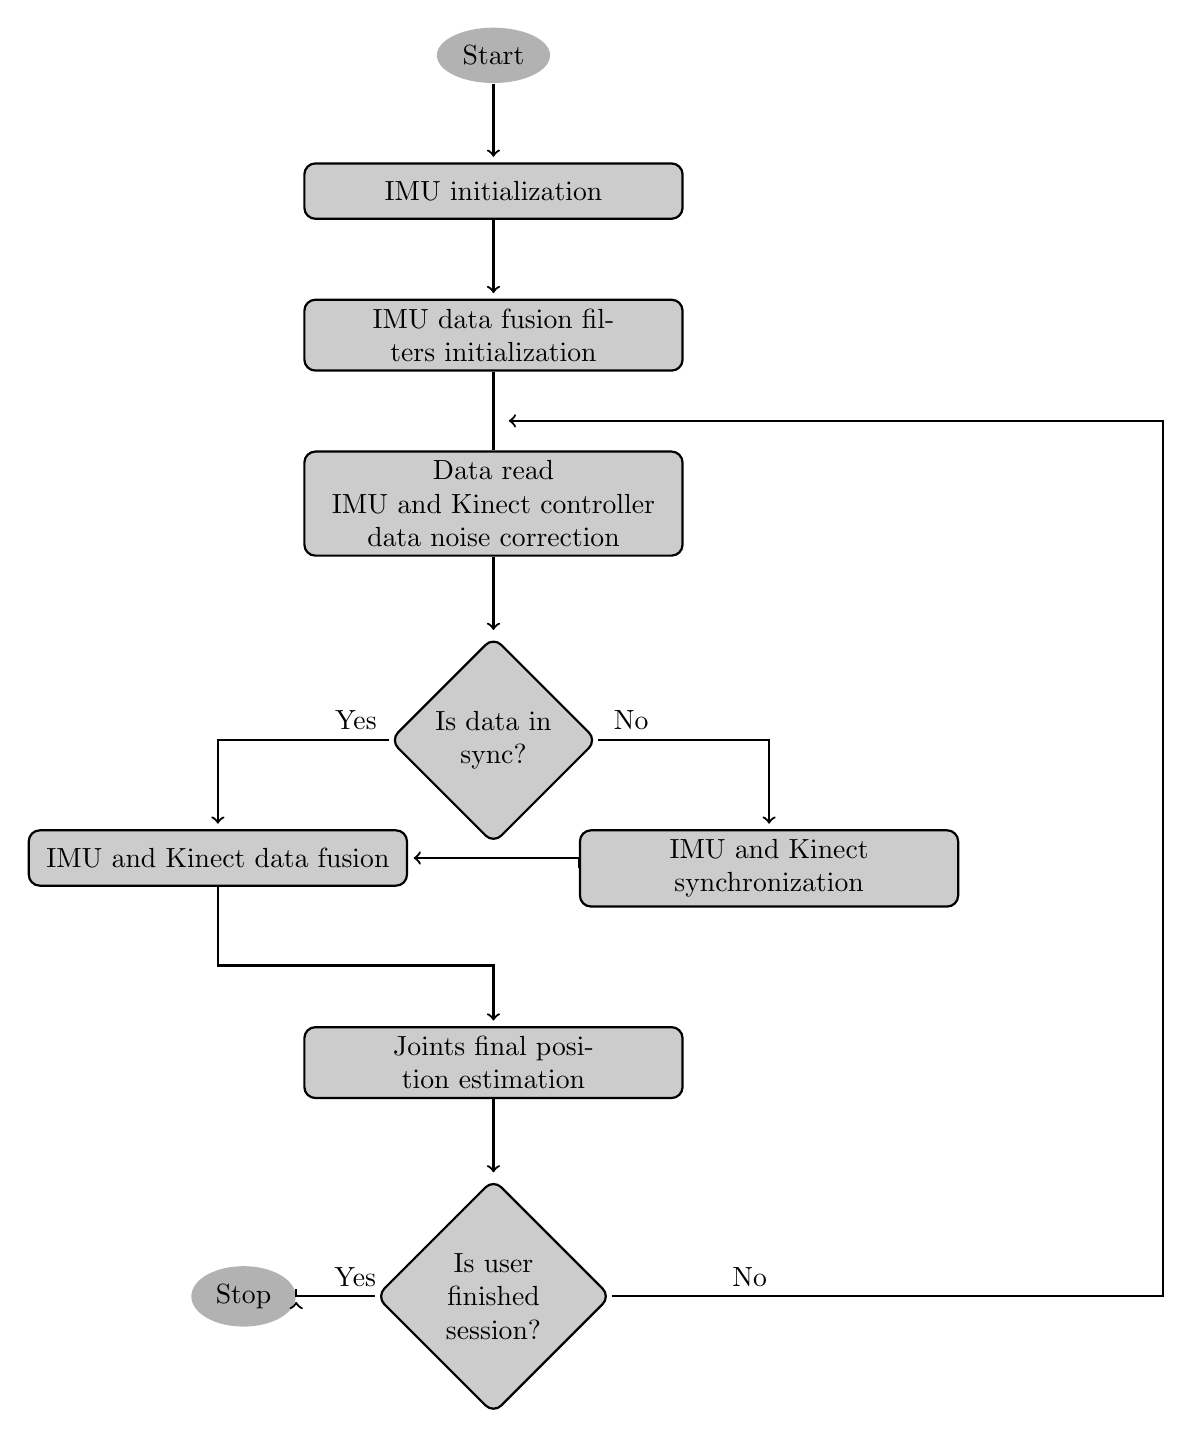
\begin{tikzpicture} [		
		auto,
		start/.style = {ellipse,fill=black!30, minimum height=2em},
		decision/.style = { diamond, draw=black, thick, fill=black!20,
			text width=5em, text badly centered,
			inner sep=1pt, rounded corners },
		block/.style    = { rectangle, draw=black, thick, 
			fill=black!20, text width=13em, text centered,
			rounded corners, minimum height=2em },
		line/.style     = { draw, thick, ->, shorten >=2pt },
	]
	% Define nodes in a~matrix
	\begin{scope} 
		\node [start] (start) {Start};
		\node [block, below=of start] (block1) {IMU initialization};
		\node [block, below=of block1] (block2) {IMU data fusion filters initialization}; 
		\node [block, below=of block2] (block7) {Data read\\IMU and Kinect controller data noise correction}; 
		\node [above=of block7, below, yshift=-0.5cm](null1) {};  					
		\node [decision, below=of block7] (inSync) {Is data in sync?}; 
		\node [block, below=of inSync, xshift=3.5cm, yshift=1.2cm] (block4) {IMU and Kinect synchronization}; 
		\node [block, below=of inSync, xshift=-3.5cm, yshift=1.2cm] (block5) {IMU and Kinect data fusion}; 
		\node [block, below=of inSync, yshift=-1.3cm] (block6) {Joints final position estimation};    
		\node [decision, below=of block6] (isEnd) {Is user finished session?}; 
		\node [start, left=of isEnd] (stop) {Stop};
	\end{scope}
	% connect all nodes defined above
	\begin{scope} [every path/.style=line]
		\path (start)        --    (block1);
		\path (block1)        --    (block2);
		\path (block2)      -- (block7) --  (inSync);
		\path (inSync)  --++  (-3,0) node [near start, above] {Yes} -| (block5.north);
		\path (inSync)  --++  (3,0) node [near start, above] {No} -| (block4.north);
		\path (block5.south)   --++  (0,-1) node {}  -|    (block6.north);
		\path (block4.west) |- (block5.east);
		\path (block6) -- (isEnd);
		\path (isEnd.east)      --++  (7,0) node [near start, above] {No} |-  (null1);
		\path (isEnd.west) --++  (-1,0) node [near start, above] {Yes} -- (stop.east);
	\end{scope}			
\end{tikzpicture}
			}
			\caption{Orientation based data fusion method schema}
			\label{fig:methodPhases}
          \end{figure}
      \end{minipage}
      	\hfill
      \begin{minipage}[b]{0.45\linewidth}
          \begin{figure}[H]
            \includegraphics[width=0.8\textwidth]{Figure11.png}
			\caption{The hand joint simplified hierarchical model}		
			\label{fig:hybrid:jointsHierarchy}	
          \end{figure}
      \end{minipage}
  \end{minipage}
	
	The discussed novel data fusion method can be presented as a formula in eq. \ref{eq:fusion:formula}.
	
	\begin{equation}
		P^F_{j,t} = f(A,G,T,P_{j-1,t}^K,P_{j,t}^K,\Delta t, P^F_{j-1,t}, P^K_{sh_L,t},P^K_{sh_R,t},l) 
		\label{eq:fusion:formula}
	\end{equation}
	
The estimation of the selected joint $j$ position ($P^F_{j,t}$) in particular time $t$ is based on the measurements of the accelerometer ($A=[a_x,a_y,a_z]$), the gyroscope ($G=[g_x,g_y,g_z]$) and the positions of the selected joint and its parent, measured by the Kinect controller ($P^K_{j,t} = [p^K_{j,x}, p^K_{j,y}, p^K_{j,z}]_t$, $P^K_{j-1,t} = [p^K_{j,x}, p^K_{j,y}, p^K_{j,z}]_t$). Additionally, to compensate IMU measurements, the current operating temperature $T$ is taken into consideration. The discussed method estimates the joint position with some time interval $\Delta t$ aligned to Microsoft Kinect update interval. IMU are sticked to the body surface, on the bone between the tracked joint $j$ and its parent joint $j-1$. The simplified hierarchical model of the hand, as well as the placement of IMU are presented in fig. \ref{fig:hybrid:jointsHierarchy}.	
	
	\subsubsection{IMU initialization}
	The goal of the IMU initialization procedure presented in the fig. \ref{fig:hybrid:IMUCalibration} is to calculate the data ($G, A$) correction factors matrix ($cor = [cor_A \quad cor_G]^T = [[c_ax,c_ay,c_az ]\quad[c_gx,c_gy,c_gz ]]^T $) for each IMU individually. 

		\begin{figure}[!htb]
	\scalebox{0.55}{		
		\input{calibrationAlgorithm.tex}
	}
	\caption{Diagram of IMU initialization routine}
	\label{fig:hybrid:IMUCalibration}
\end{figure}

	During this calculation, IMU modules must lay down without any motion, in the face-up position, as this is the position, in which we know exactly the expected data ($A_0=[0,0,1]$ for the accelerometer and $G_0=[0,0,0]$ for the gyroscope). However, the ideal values are impossible to achieve due to the noise that cannot be completly removed. Because of that, the calibration routine works iteratively ($s$ -- iteration index) as long as the average IMU measurement errors ($[\overline{A}\quad \overline{G}]^T = [[\overline{a_x},\overline{a_y},\overline{a_z}]\quad[\overline{g_x},\overline{g_y},\overline{g_z}]]^T$) are lower than the defined threshold ($[A_{th}\quad G_{th}]^T = [[a_{x,th},a_{y,th},a_{z,th}]\quad[g_{x,th},g_{y,th},g_{z,th}]]^T$). In this case, a relation of $[\overline{A}\quad \overline{G}]^T \le [A_{th}\quad G_{th}]^T$ is true when each element of the first matrix is lower than the element of the second matrix with exactly the same index. As a result of this calibration method, the matrix $cor$ is calculated, which elements added to the current IMU data, allow to use data with the desired accuracy. 
	
	If $[A\quad G]_{s,i}$ is an $i$--th out of the $n$ consecutive IMU device measurements for the iteration $s$, then the average error $[\overline{A}\quad \overline{G}]^T$ is calculated according to eq. \ref{eq:hybrid:IMUCalibration:1}.
	
	\begin{equation}
		\begin{bmatrix} \bar{A} \\ \bar{G} \end{bmatrix}_s =
		\begin{cases}
			\frac{1}{n}\sum_{i=1}^{n}{\begin{bmatrix}A \\ G\end{bmatrix}_{s,i}} & s = 1\\
			\frac{1}{n}\sum_{i=1}^{n}{\begin{bmatrix}A \\ G\end{bmatrix}_{s,i} - \begin{bmatrix}cor_A\\ cor_G\end{bmatrix}_{s-1}} &  s > 1
		\end{cases}
		\label{eq:hybrid:IMUCalibration:1}
	\end{equation}

	Then, the data correction factors matrix $cor$ for single measurement is defined by the equ. \ref{eq:hybrid:IMUCalibration:2}
	
	\begin{equation}
		\footnotesize
		cor_s = \begin{bmatrix}cor_A\\ cor_G\end{bmatrix}_s =
		\begin{cases}
			\frac{1}{8}\left(\begin{bmatrix}A_0                                                                          \\ G_0\end{bmatrix} - \begin{bmatrix}\bar{A}\\ \bar{G}\end{bmatrix}_1\right) & s = 1\\
			cor_{s-1} - diag(1/a_{x,th},1/a_{y,th},1/a_{z,th},1/g_{x,th},1/g_{y,th},1/g_{z,th}) \left(\begin{bmatrix}A_0 \\ G_0\end{bmatrix} - \begin{bmatrix}\bar{A}\\ \bar{G}\end{bmatrix}_1\right) & s > 1
		\end{cases}
		\label{eq:hybrid:IMUCalibration:2}
	\end{equation}	
	
	\subsubsection{IMU data fusion filters initialization}
	The Madgwick filter \cite{Madgwick2011}, defined with the formula presented in eq. \ref{eq:hybrid:madgwick}, has been used as an IMU module inherent accelerometer and gyroscope data fusion method. 
	
	\begin{equation}
		Q^I=m(A,G,f_m,\Delta t)
		\label{eq:hybrid:madgwick}
	\end{equation}
	
	This filter estimates the IMU module orientation in the quaternion form ($Q^I$), using accelerometer data ($A$), gyroscope data ($G$) and the filtration factor ($f_m$) based on the gyroscope drift characteristics. The Madgwick filter processes the IMU data with the time interval $\Delta t$. Before the filter can run on the real data, it needs to be initialized to set up its internal parameters correctly. The Madgwick filter initialization requires to run the filter multiple times on the measurements of not-moving accelerometer and gyroscope sensors. During this initialization the filtration factor $f_m$ needs to be set to the relatively high value i.e. 2. After the completion of the initialization process, $f_m$ should be defined according to the average Angle Random Walk (ARW) noise value $\widetilde{\omega}$ that can be calculated with the Allan’s variance\cite{FreescaleSemiconductor2015,Allan1966,Allan1987}. In case of exploited MPU-6050, IMU modules filtration factor $f_m$ is calculated according to the original article \cite{Madgwick2011} equation: $f_m = \sqrt{\frac{3}{4}\widetilde{\omega}}$, and equals $0.082$. 
	
	\subsubsection{IMU and Kinect controller data noise correction}
	The data noise correction is a crucial phase for the data fusion. Its goal is to remove as much noise as possible from the raw data. All methods used in this phase are related to measurement devices characteristics described earlier in this article.\\
	The first step to improve the IMU module data quality is the accelerometer measurements ($A$) error compensation due to the device operating temperature ($T$). For the neutral temperature ($T_0=25\degree C$) and the correction factor $f_T= 0.0011$, the correction is defined with eq. \ref{eq:hybrid:tempCorrection}. The value of $f_T$ has been estimated in self-conducted experiments.
	
	\begin{equation}
		A'=A/(1+ f_T (T-T_0))
		\label{eq:hybrid:tempCorrection}
	\end{equation}
	Low and high pass filtration of accelerometer and gyroscope data, is a part of the Madgwick filter implementation, so there is no necessity to repeat this process.
	The second measurement device – Kinect controller – requires two data correction steps that need to be performed in order to improve the measurement quality: the correction of the distance estimation and smoothing the joints position estimations. The distance estimation correction is done by the function presented in eq. \ref{eq:hybrid:distanceCorrection}, which is the opposite of the distance estimation error model (eq. \ref{eq:kinect:distanceErrorModel}). The argument of this function ($z$) is directly taken from the Kinect’s distance estimation API.
	\begin{equation}
		f(z)=z'=-0.02z^3+0.11z^2-0.27z+0.25
		\label{eq:hybrid:distanceCorrection}
	\end{equation}
	Smoothing of the Kinect’s joints positions ($P_{j,t}^K$) is necessary as coordinates fluctuations may happen, especially when occlusions occur. While there is an occlusion, positions of the same joints in two consecutive frames (measurements) can differ few centimeters, which is physically and anatomically impossible, while refresh rate of the Kinect is 30Hz. Smoothing can be done by the Kinect’s firmware, but this approach gives a significant delay of the signal interpretation. The alternative approach to smoothing positions, which was exploited in the method, was a simple low pass filter. The method used the 1st order exponential filter to remove unreliable positions estimations defined with eq. \ref{eq:hybrid:positionCorrection} and filtration factor $f_{LPF} = 0.065$.
	\begin{equation}
		{P'}_{j,t}^K=f_{LPF} * P_{j,t}^K+(1-f_{LPF}) * {P'}_{j,t-1}^K
		\label{eq:hybrid:positionCorrection}
	\end{equation}
	
	\subsubsection{IMU and Kinect synchronization}
	The data fusion of any two signals requires signals alignment in the time domain. This guarantees fusion of samples that were collected in the same time -- synchronically. The goal of IMU and Kinect signals synchronization is to find the time offset $\tau$ between two data streams. To synchronize both signals, they must have the same frequency, so the IMU signal has to be downsampled from 100Hz to 30Hz, which is a nominal frequency of the Kinect controller. The downsampling has been implemented in the form of decimation, where Kinect’s new sample availability defines the time of IMU sample picking. Then, the time offset $\tau$ between the IMU signal $I$ and the Kinect signal $K$ was defined as a time offset argument of the cross-correlation algorithm that gives the maximum value of correlation between these two signals (variable $\tau_{max}$) (eq. \ref{eq:cross-cor:1} and \ref{eq:cross-cor:2}). The value of $\tau_{max}$ is added to the timestamp of IMU samples to align it to the Kinect’s signal.
	
	\begin{subequations}
		\begin{align}
			(I \ast K)(\tau) & = \int_{-\infty}^{+\infty}I(t)K(t+\tau)dt\label{eq:cross-cor:1}   \\
			\tau_{max}       & = \underset{\tau}{argmax}((I \ast K)(\tau))\label{eq:cross-cor:2} 
		\end{align}
		\label{eq:cross-cor}
	\end{subequations}
	
	
	
	\subsubsection{IMU and Kinect data fusion}
	The data fusion method processes time aligned filtered data and takes into consideration their reliability. The most serious concerns about the quality of data, used within fusion, were related to the data provided by Microsoft Kinect controller. Decision about Kinect’s data quality was based on the several information gathered during the motion. The first one are joints tracking state combined together with their positions estimation noise level. Fully visible joint has its state set to \emph{Tracked} value and its position can be considered as reliable. Otherwise, if the tracking state value is set to \emph{Interferred}, the position estimation noise level must be calculated to check if the value can be treated as reliable or not. In the \emph{Interferred} state, the position of joint is estimated basing more on the predication than direct measurements, so its accuracy might be low and values may differ significantly between consequitive frames (or in short time period). Other parameters taken into consideration are the value of angle $\alpha$ between the user and the camera, and information about tracking state of both shoulder joints. Microsoft Kinect has been designed to track the motion of human who stand frontally to the camera. If user rotate too much, Kinect is not able to track the motion correctly anymore. During self experiments, it turned that the maximum angle between human and the Kinect is $50\degree$. Exceeding this rotation angle value results in unreliable, often random, values of all joints positions. As the the value of angle $\alpha$ is calculated using position values of both shoulder joints, they both should be fully visible (tracking state set to \emph{Tracked}), and their position values estimations should be stable in time. That means the angle measurement variance should be lower than $1.5\degree$, which means there were no rapid changes in shouldes position estimations characteristic for signifiant error in provided data. 
	
	If all mentioned conditions were satisfied, signals were fused according to equation \ref{eq:hybrid:reliableFusion}. The novelty of the presented method, in comparison with literature approaches, is that the fused data represents skeleton bones orientations in the form of Euler angles $E = \begin{bmatrix} \phi &  \theta & \psi \end{bmatrix}$, instead of joints resulting positions. Orientations of the bones are estimated from both sources and are represented in form of quaternions. They must be converted to the form of Euler angles before they are fused. The conversion from quaternion to Euler angles form can be found in \cite{Dunn2011}.
	
	\begin{equation} E^F_t = 
		\begin{bmatrix}  \phi^F \\  \theta^F \\  \psi^F \end{bmatrix}_t = 
		diag(w_\phi,w_\theta,w_\psi)
		\begin{bmatrix}  \phi^I \\  \theta^I \\  \psi^I \end{bmatrix}_t + 
		diag(1-w_\phi,1-w_\theta,1-w_\psi)
		\begin{bmatrix}  \phi^K \\  \theta^K \\  \psi^K \end{bmatrix}_t
		\label{eq:hybrid:reliableFusion}
	\end{equation}
	
	The originally elaborated weights $[w_\phi , w_\theta , w_\psi]$ describe the importance level of IMU measurements. They were based both on the device precision and data completeness, and were defined as $[0.98, 0.05, 0.65]$ respectively. 
	
	If Kinect’s data turns out to be unreliable, they cannot be fused with the IMU data. Averaged bones orientation are then estimated based on the previously ($t-1$) fused estimation and current change of IMU orientation, according to equation \ref{eq:hybrid:unreliableFusion}.
	
	
	\begin{equation} 
		\label{eq:hybrid:unreliableFusion}
		E^F_t = 
		\begin{bmatrix}  \phi^F \\  \theta^F \\  \psi^F \end{bmatrix}_t = 
		\begin{bmatrix}  \phi^F \\  \theta^F \\  \psi^F \end{bmatrix}_{t-1} +
		diag(w_\phi,w_\theta,w_\psi)\
		(\begin{bmatrix}  \phi^I \\  \theta^I \\  \psi^I \end{bmatrix}_t -
		\begin{bmatrix}  \phi^I \\  \theta^I \\  \psi^I \end{bmatrix}_{t-1})
	\end{equation}
	
	However, in case of Kinect data unreliability, weights $[w_\phi , w_\theta , w_\psi]$ were defined differently. In equation \ref{eq:hybrid:unreliableFusion} these weights were defined as $$[0.98,(1-t_{noise}/10)*0.65,(1-t_{noise}/10)*0.65]$$ where $t_{noise}$ coefficient defines the time, in seconds, that Kinect stayed unreliable and its maximum accepted value was defined to 10s. After this time, estimation of the new bone orientation (only around two axes) stops, until Kinect is available again, and the method privileges the IMU signal.
	
	\subsubsection{Joints final position estimation}
	Final joint position ($P_{j,t}^F$) estimation requires the information regarding the position of joint’s parent in the hierarchical skeleton model ($P_{j-1,t}^F$), fixed length of the bone between current joint and its parent ($l$) and the bone orientation estimation ($E_t^F=[\phi^F,\theta^F,\psi^F]_t$). As a result of data fusion, estimated orientations were presented in the form of Euler angles. However, this representation of orientation may complicate further calculations. To simplify calculations, opposite conversion from Euler angles to quaternion $Q_t^F$, according to the formula described in \cite{Dunn2011}, is required. As the used skeletal model is defined as a herarchical structure, newly estimated joint position must be aligned to the postion of its parent joint. Taking tht into consideration, the final joint position calculation procedure is described with equation \ref{eq:hybrid:positionCalculationForm}.
	
	\begin{equation} 	
		P_{j,t}^F=P_{j-1,t}^F+Q_t^F*[l,0,0]*{Q_t^F}^{-1}     
		\label{eq:hybrid:positionCalculationForm}              	
	\end{equation}
	
	%%%%%%%%%%%%%%%%%%%%%%%%%%%%%%%%%%%%%%%%%%
	\section{Results}
	
	%This section may be divided by subheadings. It should provide a concise and precise description of the experimental results, their interpretation as well as the experimental conclusions that can be drawn.
	
	In order to verify the accuracy of elaborated method, several experiments were performed. They were conducted with the Vicon motion capture system, as a source of ground-truth reference data. For 3 subjects hand movements were monitored, being tracked simultaneously with Kinect controller, two IMU attached to hand arm and forearm bones on the skin surface, as well as Vicon tracking system. Each user had to perform 4 exercises, each of them twice with 5 repetitions per single try. Each try started with devices synchronization in the T-Pose and then 5 repetitions of motion began. Exercises focused on horizontal and vertical hand flexion in elbow joint, horizontal hand motion and keeping straight arm in T-pose without motion for at least 60s. All these exercises schemes are presented in figure \ref{fig:results:sequences}.
	
	\begin{figure}[H]
		\centering
		\includegraphics[width=12cm]{Figure8.png}
		\caption{Movement sequences performed during tests}
		\label{fig:results:sequences}
	\end{figure}
	
	The accuracy of 3 parameters estimations has been observed: the position of elbow joint, the position of wrist joint and the angle between arm and forearm measured in elbow joint. Those values have been compared with the corresponding parameters estimated with Kalkbrenner’s method \cite{Kalkbrenner2014} which, on the contrary, fused positions rather than orientations, of selected joints. The position estimation error has been defined as root mean squared error ($RMSE$) of Euclidean distance ($d_e$) between joint’s reference position, measured by Vicon motion capture system ($P_j^V$), and joint’s position estimated by two data fusion methods. The first one is the joins position-based Kalkbrenner data fusion method ($P_j^{FP}$) and the second: bones orientation-based fusion method ($P_j^{FO}$) proposed by the authors of this article. The $RMSE$ value has been calculated with equation \ref{eq:results:RMSE} \cite{Armstrong1992}. The error for elbow joint angle $\beta$ estimation has been calculated in the similar way.
	
	\begin{equation}
		{RMSE}^F_j = \sqrt{\frac{1}{n}\sum_{i=1}^{n}{d_e(P^V_{j,i}, P^{Fs}_{j,i})^2}} , s = \{O,P\}
		\label{eq:results:RMSE}
	\end{equation}
	
	The overall error of both methods, for each test exercise, has been calculated as a mean of $RMSE$ ($\overline{RMSE}$) of each motion tracking session. To compare the Kalkbrenner’s method with authors’ novel method the ratio $r$ between the difference of $\overline{RMSE}$ of both methods to the $\overline{RMSE}$ of Kalkbrenner’s method has been calculated according to the equation \ref{eq:results:comparison} and expressed in the form of percents. The figures \ref{fig:results:positionError:a} and \ref{fig:results:positionError:b} show the summary of  $\overline{RMSE}$ for tracked upper limb joints: elbow and wrist. Above each pair of bars, in these charts, the value of $r$ ratio has been presented. Based on the results, presented in figures \ref{fig:results:positionError:a} and \ref{fig:results:positionError:b}, the improvement of proposed bones orientation-based fusion method, in reference to the best in literature -- Kalkbrenner’s method has been noticed. However, the improvement ratio vary between joints. The error of the elbow joint position estimation has been reduced up to 18\% and the wrist joint position estimation error -- up to 16\%. The difference in improvement ration between these two joints is caused by the fact that elbow joint is closer to the skeleton model root than wrist joint, so it accumulates less asceding joints position estimations errors. Figure \ref{fig:results:elbowAngleError} presents the chart of $\overline{RMSE}$ of elbow angle $\beta$ estimation (calculated similarly to eq. \ref{eq:results:RMSE}). In this value estimation the improvement has been also noticed and its ratio is up to 11\%.
	
	\begin{equation}
		r = \frac{\overline{RMSE^P_j} - \overline{RMSE^O_j}}{\overline{RMSE^P_j}}
		\label{eq:results:comparison}
	\end{equation}
	
	\begin{figure}[H]
		\centering
		\begin{subfigure}[b]{0.49\textwidth}
			\centering
			\input{Figure9a.tex}
			\caption{Elbow}
			\label{fig:results:positionError:a}
		\end{subfigure} \hfill
		\begin{subfigure}[b]{0.49\textwidth}
			\centering
			\input{Figure9b.tex}
			\caption{Wrist}
			\label{fig:results:positionError:b}
		\end{subfigure}
		\caption{Average root square mean error $\overline{RMSE}$ of elbow (a) and wrist (b) joints position estimation}
		\label{fig:results:positionError}
	\end{figure}   
	
	\begin{figure}[H]
		\centering
		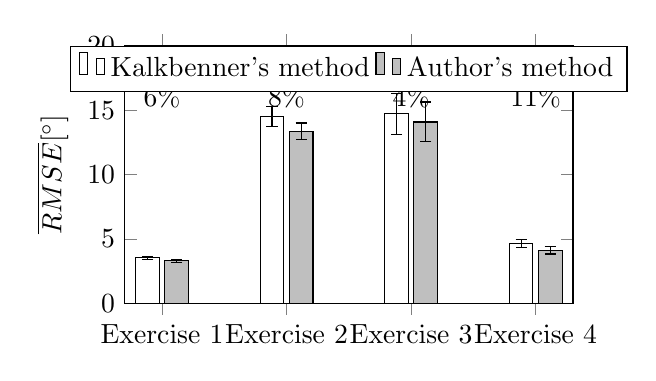
\begin{tikzpicture}
	\begin{axis}[
			ybar,
			bar width=.3cm,
			width=.6\textwidth,
			height=.4\textwidth,
			legend style={at={(0.5,1)},
				anchor=north,legend columns=-1},
			symbolic x coords={ex 1,ex 2,ex 3,ex 4},
			xtick=data,
			xticklabels={Exercise 1,Exercise 2,Exercise 3,Exercise 4},
			ymin=0,ymax=20,
			ylabel={$\overline{RMSE} [\degree]$},
		]
		\addplot [black,fill=white,error bars/.cd,y dir=both,y explicit] coordinates { 
			(ex 1,3.54) +- (0.0, 0.12)
			(ex 2,14.49) +- (0.0, 0.77)
			(ex 3,14.71) +- (0.0, 1.57)
			(ex 4,4.65)  +- (0.0, 0.32)
		};
		\addplot [black,fill=black!25,error bars/.cd,y dir=both,y explicit] coordinates { 
			(ex 1,3.29) +- (0.0, 0.12)
			(ex 2,13.35)+- (0.0, 0.65)
			(ex 3,14.08)+- (0.0, 1.55)
		(ex 4,4.11)  +- (0.0, 0.29)};
																															
		\legend{Kalkbenner's method, Author's method}
		\node at (axis cs:ex 1,16){\textcolor{black}{6\%}};
		\node at (axis cs:ex 2,16){\textcolor{black}{8\%}};
		\node at (axis cs:ex 3,16){\textcolor{black}{4\%}};
		\node at (axis cs:ex 4,16){\textcolor{black}{11\%}};
	\end{axis}
\end{tikzpicture}	
	
		\caption{Average root square mean error $\overline{RMSE}$ of elbow flexion angle $\beta$}
		\label{fig:results:elbowAngleError}
	\end{figure}
	
	%%%%%%%%%%%%%%%%%%%%%%%%%%%%%%%%%%%%%%%%%%
	\section{Discussion}
	
	%Authors should discuss the results and how they can be interpreted in perspective of previous studies and of the working hypotheses. The findings and their implications should be discussed in the broadest context possible. Future research directions may also be highlighted.
	The presented results show the comparison of estimation errors of two data fusion methods: the well-known method based on joints positions fusion and a new data fusion method based on bones orientations. 3 parameters estimated by both methods: elbow joint position, wrist joint position and elbow angle $\beta$, have been taken into consideration in this comparison: the error of elbow joint position estimation, the error of wrist joint position estimation and the error of the estimation of angle between the arm and the forearm of the tracked hand. The set of motions, used to test these methods, have been chosen to check how methods work when source data are poor quality due to the limitations and imperfections of measurement devices.
	
	The results of error comparison for elbow and wrist joints positions estimations are presented in figures \ref{fig:results:positionError:a} and \ref{fig:results:positionError:b} respectively. Results proof that the author’s novel data fusion method reduces the joints position estimation error, especially during motions that emphasize the imperfections of Microsoft Kinect device (exercises 2 and 3). In controller demanding motions, the most significant improvement, in estimation error, has been noticed - up to 18\% for the elbow position estimation and up to 16\% for the wrist position estimation. In two other motions, the improvement has been noticed as well, however it was slightly less substantial than in the exercises 2 and 3. This shows that the presented orientation-based data fusion method is able to detect the poor Kinect data quality faster than the method proposed by Kalkbrenner and reduce the influence of these data on the selected joint position estimation. 
	
	Figure \ref{fig:results:elbowAngleError} shows the results of the elbow angle estimation during the motion. In this parameter, the estimation error reduction has been noticed as well, and the best improvement was close to 11\%. However, in exercises 2 and 3, which might be considered as the most difficult from the data quality detection point of view, the improvement is slighter than in the case of joints position estimation. That means that both methods have similar accuracy of estimation of the body/limbs shape, however, the authors’ method is more accurate in the joints position estimation. The most possible explanation for this, is the fact that the authors’ method uses the fixed bones length definition,while the Kalkbrenner’s method uses the Kinect’s bone length temporary estimation that may vary between subsequent measurement frames.
	
	%%%%%%%%%%%%%%%%%%%%%%%%%%%%%%%%%%%%%%%%%%
	\section{Conclusions}
	
	%This section is not mandatory, but can be added to the manuscript if the discussion is unusually long or complex.
	
	The authors presented a new, orientation-based method for skeleton joints positioning, that compensates devices' imperfections and considers the context of the motion. It was tested on a set of right hand movements demanding for measurement devices. Results were compared with those gathered from the position-based fusion method and the reference, professional, ground-truth Vicon tracking system. With the results achieved from the experiments, one can notice the improvement of the elbow positioning accuracy up to 18\%, the wrist positioning up to 16\% and the elbow joint angle estimation accuracy up to 11\%.
	Obtained results prove that the novel data fusion approach, based on the bones orientation, might be considered as an improved alternative to the well-known, joint position-based methods.
	
	
	%%%%%%%%%%%%%%%%%%%%%%%%%%%%%%%%%%%%%%%%%%
	\vspace{6pt} 
	
	%%%%%%%%%%%%%%%%%%%%%%%%%%%%%%%%%%%%%%%%%%
	%% optional
	%\supplementary{The following are available online at www.mdpi.com/link, Figure S1: title, Table S1: title, Video S1: title.}
	
	%%%%%%%%%%%%%%%%%%%%%%%%%%%%%%%%%%%%%%%%%%
	%\acknowledgments{All sources of funding of the study should be disclosed. Please clearly indicate grants that you have received in support of your research work. Clearly state if you received funds for covering the costs to publish in open access.}
	
	%%%%%%%%%%%%%%%%%%%%%%%%%%%%%%%%%%%%%%%%%%
	\authorcontributions{G. Glonek designed the method and experiments and analyzed the data; A.Wojciechowski contributed and supervised the work; G. Glonek and A. Wojciechowski wrote the paper.}
	
	%%%%%%%%%%%%%%%%%%%%%%%%%%%%%%%%%%%%%%%%%%
	\conflictofinterests{The authors declare no conflict of interest.} 
	
	%%%%%%%%%%%%%%%%%%%%%%%%%%%%%%%%%%%%%%%%%%
	%% optional
	\abbreviations{The following abbreviations are used in this manuscript:\\
						
		\noindent 
		\begin{tabular}{@{}ll}
			RMSE & Root Mean Squared Error    \\
			IMU  & Inertial Measurement Units \\
			LPF  & Low Pass Filter            \\
		\end{tabular}}
	
	%%%%%%%%%%%%%%%%%%%%%%%%%%%%%%%%%%%%%%%%%%
	%% optional
	%\appendixtitles{no} %Leave argument "no" if all appendix headings stay EMPTY (then no dot is printed after "Appendix A"). If the appendix sections contain a heading then change the argument to "yes".
	%\appendixsections{multiple} %Leave argument "multiple" if there are multiple sections. Then a counter is printed ("Appendix A?). If there is only one appendix section then change the argument to ?one? and no counter is printed (?Appendix?).
	%\appendix
	%\section{}
	%The appendix is an optional section that can contain details and data supplemental to the main text. For example, explanations of experimental details that would disrupt the flow of the main text, but nonetheless remain crucial to understanding and reproducing the research shown; figures of replicates for experiments of which representative data is shown in the main text can be added here if brief, or as Supplementary data. Mathemtaical proofs of results not central to the paper can be added as an appendix.
	
	%\section{}
	%All appendix sections must be cited in the main text. In the appendixes, Figures, Tables, etc. should be labeled starting with `A', e.g., Figure A1, Figure A2, etc. 
	
	%%%%%%%%%%%%%%%%%%%%%%%%%%%%%%%%%%%%%%%%%%
	% Citations and References in Supplementary files are permitted provided that they also appear in the reference list here. 
	\bibliographystyle{mdpi}
	
	%=====================================
	% References, variant A: internal bibliography
	%=====================================
	%\renewcommand\bibname{References}
	%\begin{thebibliography}{999}
	% Reference 1
	%\bibitem{ref-journal}
	%Lastname, F.; Author, T. The title of the cited article. {\em Journal Abbreviation} {\bf 2008}, {\em 10}, 142-149.
	% Reference 2
	%\bibitem{ref-book}
	%Lastname, F.F.; Author, T. The title of the cited contribution. In {\em The Book Title}; Editor, F., Meditor, A., Eds.; Publishing House: City, Country, 2007; pp. 32-58.
	%\end{thebibliography}
	
	%=====================================
	% References, variant B: external bibliography
	%=====================================
	\bibliography{main}
	
	%%%%%%%%%%%%%%%%%%%%%%%%%%%%%%%%%%%%%%%%%%
	%% optional
	%\sampleavailability{Samples of the compounds ...... are available from the authors.}
	
	%%%%%%%%%%%%%%%%%%%%%%%%%%%%%%%%%%%%%%%%%%
\end{document}

